\documentclass[UTF8]{article}
%\usepackage[left=2.50cm, right=2.50cm, top=2.50cm, bottom=2.50cm]{geometry}
\usepackage[margin=1in]{geometry}

% -- text font --
% compile using Xelatex
%\setmainfont{Microsoft YaHei}  % 微软雅黑
%\setmainfont{YouYuan}  % 幼圆    
%\setmainfont{NSimSun}  % 新宋体
%\setmainfont{KaiTi}    % 楷体
%\setmainfont{SimSun}   % 宋体
%\setmainfont{SimHei}   % 黑体

\usepackage{times}
%\usepackage{mathpazo}
%\usepackage{fourier}
%\usepackage{charter}
%\usepackage{helvet}

\usepackage{amsfonts,amsmath,amssymb} 
\usepackage[none]{hyphenat} 
\usepackage{fancyhdr} 
\usepackage{fontspec, xeCJK} 
\setCJKmainfont{SimSun}
\usepackage{indentfirst}
%\CJKindent
\setlength{\parskip}{10pt}
%\setlength{\parindent}{10pt}


\usepackage[english]{babel}
\usepackage{color}      % color content
\usepackage{graphicx}   % import figures
\usepackage{url}        % hyperlinks
\usepackage{bm}         % bold type for equations
\usepackage{multirow}
\usepackage{booktabs}
\usepackage{epstopdf}
\usepackage{epsfig}
\usepackage{algorithm}
\usepackage{algorithmic}
\renewcommand{\algorithmicrequire}{ \textbf{Input:}}     % use Input in the format of Algorithm  
\renewcommand{\algorithmicensure}{ \textbf{Initialize:}} % use Initialize in the format of Algorithm  
\renewcommand{\algorithmicreturn}{ \textbf{Output:}}     % use Output in the format of Algorithm  
\pagestyle{fancy}
\fancyhead{}
\fancyfoot{}

\begin{document}
\begin{titlepage}
    \begin{center}
        \vspace*{1cm}
        \Large{\textbf{2017}}\\
        \Large{\textbf{应用数学}}\\
        \vfill
        \line(1,0){400}\\[1mm]
        \huge{\textbf{论文阅读报告}}\\
        \Large{\textbf{R-Net}}\\
        \line(1,0){400}\\
        \vfill
        By 孙付\\
        17210240013\\
        \today\\
    \end{center}
\end{titlepage}
\section{问题描述}
SQuAD数据集是斯坦福大学发布的公开数据集,提供train和dev训练集,未公开test数据集。该数据集上的数据给定一段passage和一个Question,求取Answer,Answer为文中出现的一个东西,Passage、Question 和Answer对如下所示。
\begin{quotation}
\noindent Passage: Tesla later approached Morgan to ask for more funds to build a more powerful transmitter.  When asked where all the money had gone, Tesla responded by saying that he was affected by the Panic of 1901, which he (Morgan) had caused. Morgan was shocked by the reminder of his part in the stock market crash and by Tesla’s breach of contract by asking for more funds. Tesla wrote another plea to Morgan, but it was also fruitless. Morgan still owed Tesla money on the original agreement, and Tesla had been facing foreclosure even before construction of the tower began.

\noindent Question: On what did Tesla blame for the loss of the initial money?

\noindent Answer: Panic of 1901
\end{quotation}
\section{模型结构}
\begin{figure}[htpb]
    \centering
    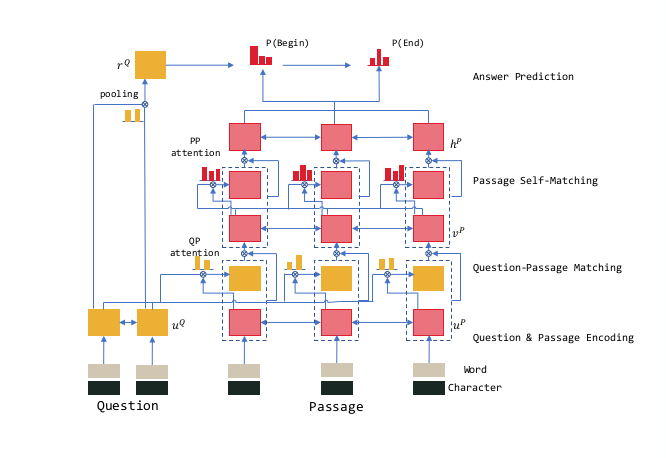
\includegraphics[width=0.8\linewidth]{r-net.png}
    \label{fig:R-Net}
    \caption{R-Net}
\end{figure}

模型看起来很复杂,其实主要就是对attention的运用,而且对attention运用了非常多的次数,个人感觉此结构对给定的passage和question进行了非常深入的挖掘,但是仅仅是对文本本身的挖掘,和语义理解没有什么关系。由于文中用到了attention来对passage和question(passage)进行match,最后用pointer networks来选择答案,所以下面对前面的文章由远到近的讲一下。
\section{Neural Machine Translation by Jointly Learning to Align and Translate}

原论文是用于解决机器翻译的问题,结构如下
\begin{figure}[htpb]
    \centering
    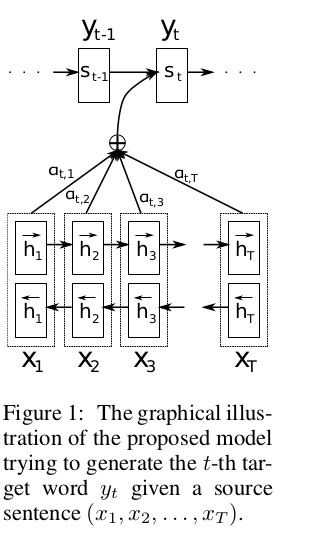
\includegraphics[width=0.5\linewidth]{attention.png}
    \label{fig:Attention}
    \caption{Attention}
\end{figure}
简单推导(本文主题不在此,简单介绍),定义条件概率:
$$p(y_i|y1,...,y_{i-1},x)=g(y_{i-1},s_i,c_i)$$
其中$s_i$是RNN的hidden state,y是翻译的输出,x是输入,$s_i$通过 $$s_i=f(s_{i-1},y_{i-1},c_i)$$
计算,向量$c_i$由处理输入的BiRNN的隐藏状态决定,
$$c_i=\sum_{j=1}^{T_x}\alpha_{ij}h_j$$,
权重$\alpha_{ij}$通过
$$\alpha_{ij}=\frac{exp(e_{ij})}{\sum_{k=1}^{T_x}exp(e_{ij})}$$
计算且$e_{ij}=a(s_{i-1},h_j)$,这个函数用于对第j个位置的输入和第i个位置的输出打分,看看他们之间有多match,原文是用一个神经网络train的,后面的用于解决QA问题的一般都是直接计算的,用一个矩阵表示。如在论文Text Understanding with the Attention Sum Reader Network中的方法:
\begin{quotation}
\noindent \begin{itemize}
    \item We compute a vector embedding of the query.

    \item We compute a vector embedding of each indi-vidual word in the context of the whole doc-ument (contextual embedding).

    \item Using a dot product between the question embedding and the contextual embedding of each occurrence of a candidate answer in the document, we select the most likely answer.
\end{itemize}
\end{quotation}

\section{Pointer Networks}

在该论文中将上面的attention的具体计算方法直接给出了,此为对第i个输出计算,$e_i$,$d_i$分别便是encoder和decoder的hidden states:
$$u_j^i=v^T\tanh(W_1e_j+W_2d_i) , j\in(1,..,n)$$
$$a_j^i=softmax(u_j^i),j\in(1,...,n)$$
$$d_i’=\sum_{j=1}^na_j^ie_j$$
第二步的softmax即将$u_j^i$转化成attention。

文中提出的Ptr-Net将attention的那一步直接替换成输入的每个token做为输出的概率,即:
$$u_j^i=v^T\tanh(W_1e_j+W_2d_i) , j\in(1,..,n)$$
$$p(C_i|C_1,...,C_{i-1},P)=softmax(u^i)$$
这种结构在解决输出的内容在输入中出现非常好用。

\section{Learning Natural Language Inference with LSTM}

\begin{figure}[htpb]
    \centering
    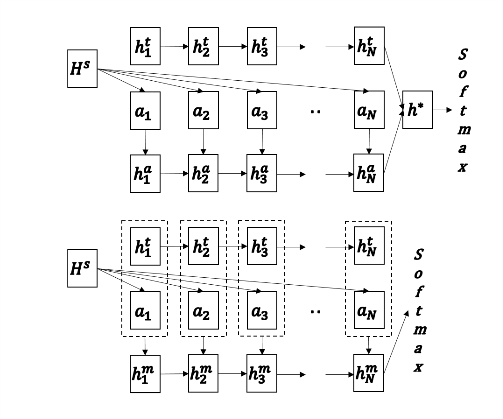
\includegraphics[width=0.7\linewidth]{Match-LSTM.png}
    \label{fig:Match-LSTM}
    \caption{Match-LSTM}
\end{figure}
fig
此文本来是用来解决natural language inference的问题的,在上半部分是前人提出的attention机制,“A dog jumping for a Frisbee in the snow.” and the hypothesis “A cat washes his face and whiskers with his front paw.” 在该句子中dog和cat不匹配,应该被记住,最后得出两个句子关系为contradiction,但是上面的结构直接由最终状态得出结论效果不好(距离太长容易忘记),所以受到lstm的启发,在向后传的时候增加了几个门,用于控制记忆和遗忘。正是用了这些门机制(和LSTM的门非常类似,这里不再写出),所以该结构称之为Match-LSTM。

\section{Machine Comprehension Using Match-LSTM and Answer Pointer}
\begin{figure}[htpb]
    \centering
    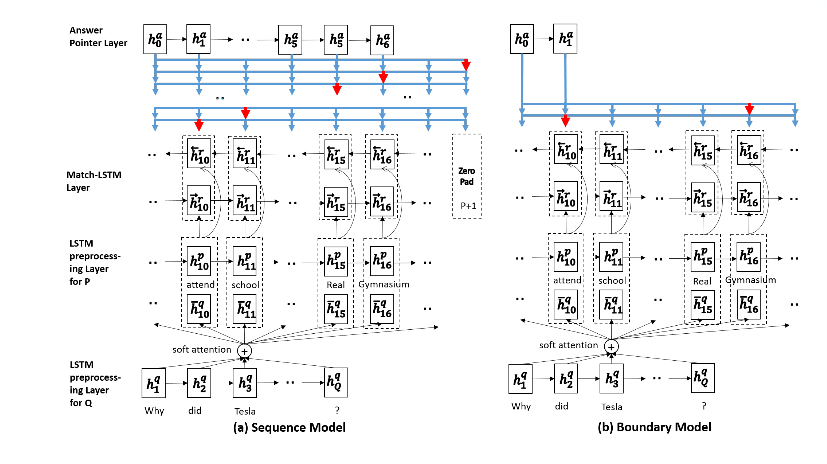
\includegraphics[width=0.8\linewidth]{m-p.png}
    \label{fig:Match-LSTM}
    \caption{Match-LSTM}
\end{figure}
上图即此论文提出的结构,最下面是将问题过一个LSTM,第二层是将原文过一次LSTM,然后通过上文提到的Match-LSTM方法处理,再通过Pointer Networks获得输出,左半边是原来的pointer networks,右边的是直接截取一个开始点和一个终止点得到答案。最终的loss function如下:
$$-\sum_{n=1}^N\log p(a_n|P_n,Q_n)$$
\section{R-Net}
\par
有了之前的铺垫,R-net就很好理解了,下面的Question-Passage Matching(QPM)就是之前提到的Match-LSTM,中间加了一个Passage Self-Matching,最后通过Pointer Networks预测输出。
\par
R-net的主要的创新点就在提出了Passage Self-Matching,因为QPM只用到了问题和文章局部信息,并未挖掘文章本身信息之间的关联,所以加入了一个self attention之后效果很好。

\end{document}

